\part{Resultados computacionais}
\label{sec:resultados}
%LOCK Galinkin

A heurística desenvolvida foi aplicada a alguns gráficos clássicos da
literatura. Para cada exemplo, serão apresentados o grafo, junto com a
CMV do mesmo. Além disso, serão apresentados três números:
\begin{description}
    \item[$n$] O número de vértices do grafo.
    \item[$k$] O número de vértices da CMV.
    \item[$k'$] O número de vértices da cobertura de vértices
    encontrada pela heurística.
\end{description}

\section{O tetraedro}
Para o tetraedro~\cite{cite:example-plato} com $n=4$ vértices.

\begin{figure}[htb]
\centering
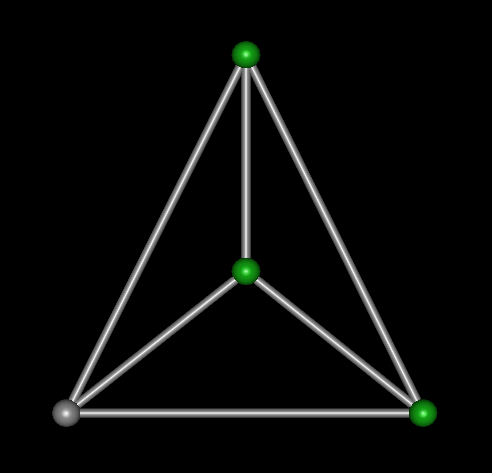
\includegraphics[width=0.4\textwidth]{img/tetraedro.png}
\label{fig:example-tetraedro}
\caption{Tetraedro, $n=4$, $k=3$}
\end{figure}

\section{O grafo bipartido de Kuratowski $K_{3,3}$}
Para o grafo bipartido de kuratowski
$K_{3,3}$~\cite{cite:example-kuratowski} com $n=6$ vértices.

\begin{figure}[htb]
\centering
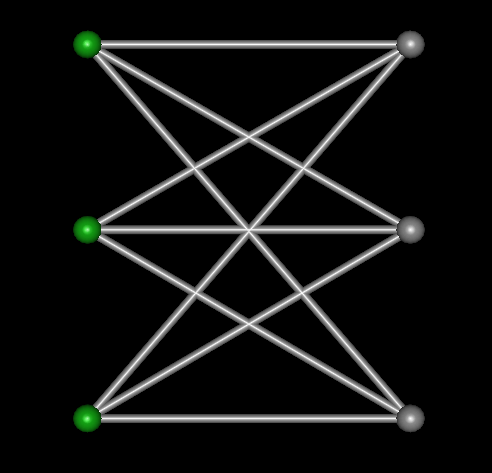
\includegraphics[width=0.4\textwidth]{img/kuratowski.png}
\label{fig:example-kuratowski}
\caption{Grafo bipartido de Kuratowski $K_{3,3}$, $n=6$, $k=3$}
\end{figure}


\section{O octaedro}
Para o octaedro~\cite{cite:example-plato} com $n=6$ vértices.

\begin{figure}[htb]
\centering
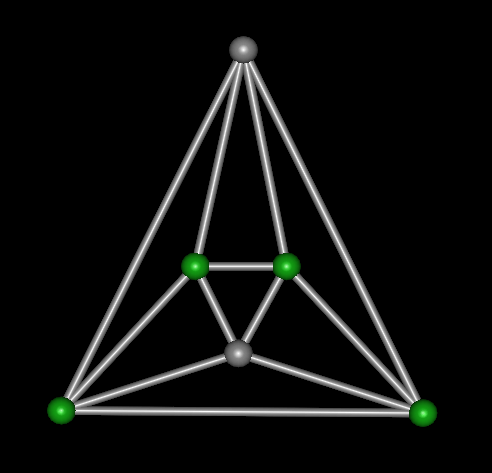
\includegraphics[width=0.4\textwidth]{img/octaedro.png}
\label{fig:example-octaedro}
\caption{Octaedro, $n=6$, $k=4$}
\end{figure}


\section{O grafo de Bondy-Murphy $G_1$}
Para o grafo de Bondy-Murphy $G_1$~\cite{cite:example-bondy} com $n=7$
vértices.

\begin{figure}[htb]
\centering
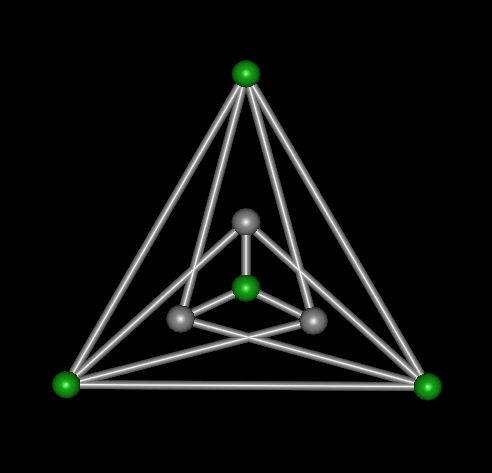
\includegraphics[width=0.4\textwidth]{img/bondymurphyg1.png}
\label{fig:example-bondymurphyg1}
\caption{Grafo de Bondy-Murphy $G_1$, $n=7$, $k=4$}
\end{figure}


\section{O grafo roda $W_8$}
Para o grafo roda $W_8$~\cite{cite:example-bondy} com $n=8$ vértices.

\begin{figure}[htb]
\centering
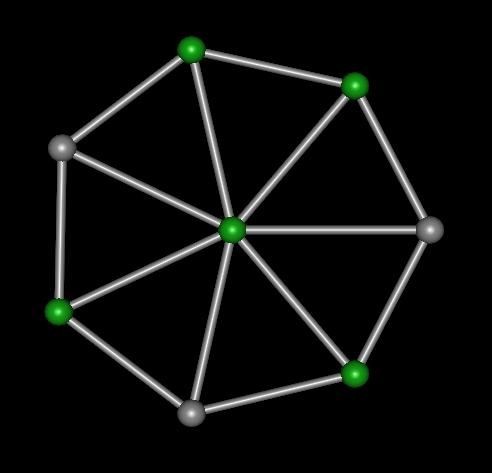
\includegraphics[width=0.4\textwidth]{img/wheel.png}
\label{fig:example-wheel}
\caption{Grafo roda $W_8$, $n=8$, $k=5$}
\end{figure}


\section{O cubo}
Para o grafo cubo~\cite{cite:example-plato} com $n=8$ vértices.

\begin{figure}[htb]
\centering
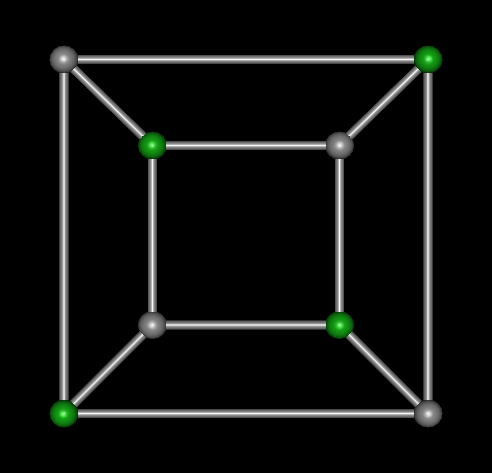
\includegraphics[width=0.4\textwidth]{img/cube.png}
\label{fig:example-cube}
\caption{Grafo cubo, $n=8$, $k=4$}
\end{figure}


\section{O grafo Petersen}
Para o grafo Petersen~\cite{cite:example-petersen} com $n=10$
vértices.

\begin{figure}[htb]
\centering
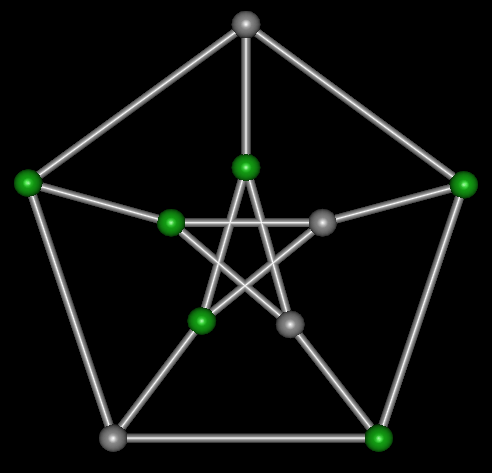
\includegraphics[width=0.4\textwidth]{img/petersen.png}
\label{fig:example-petersen}
\caption{Grafo de Petersen, $n=10$, $k=6$}
\end{figure}


\section{O grafo de Bondy-Murphy $G_2$}
Para o grafo de Bondy-Murphy $G_2$~\cite{cite:example-bondy} com $n=11$
vértices.

\begin{figure}[htb]
\centering
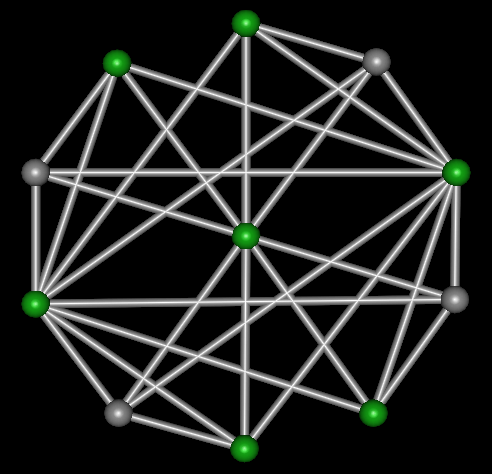
\includegraphics[width=0.4\textwidth]{img/bondymurphyg2.png}
\label{fig:example-bondymurphyg2}
\caption{Grafo de Bondy-Murphy $G_2$, $n=11$, $k=7$}
\end{figure}


\section{O grafo de Grötzsch}
Para o grafo de Grötzsch~\cite{cite:example-grotzsch} com $n=11$
vértices.

\begin{figure}[htb]
\centering
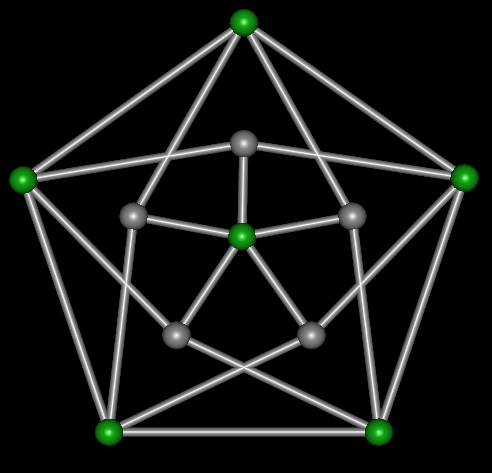
\includegraphics[width=0.4\textwidth]{img/grotzsch.png}
\label{fig:example-grotzsch}
\caption{Grafo de Grötzsch, $n=11$, $k=6$}
\end{figure}


\section{O grafo de Herschel}
Para o grafo de Herschel~\cite{cite:example-herschel} com $n=11$
vértices.

\begin{figure}[htb]
\centering
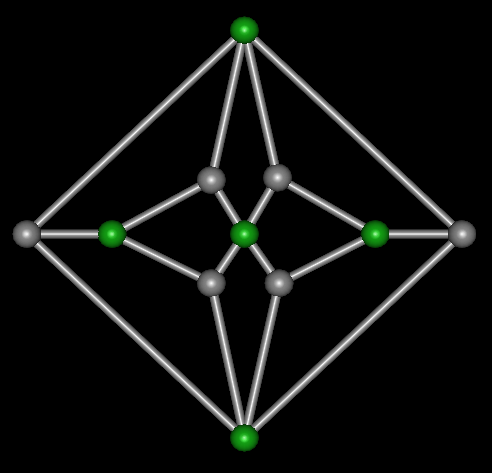
\includegraphics[width=0.4\textwidth]{img/herschel.png}
\label{fig:example-herschel}
\caption{Grafo de Herschel, $n=11$, $k=5$}
\end{figure}


\section{O icosaedro}
Para o icosaedro~\cite{cite:example-plato} com $n=12$ vértices.

\begin{figure}[htb]
\centering
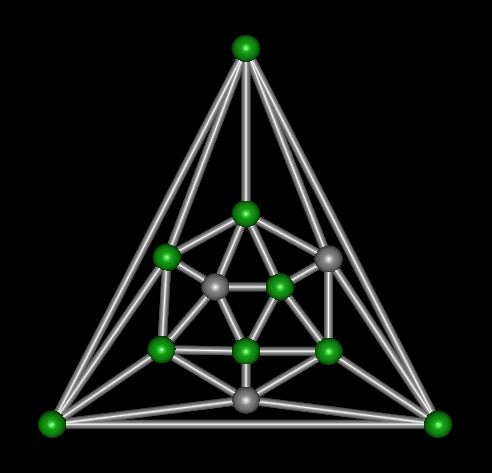
\includegraphics[width=0.4\textwidth]{img/icosaedro.png}
\label{fig:example-icosaedro}
\caption{Icosaedro, $n=12$, $k=9$}
\end{figure}


\section{O grafo de Bondy-Murphy $G_3$}
Para o grafo de Bondy-Murphy $G_3$~\cite{cite:example-bondy} com $n=14$
vértices.

\begin{figure}[htb]
\centering
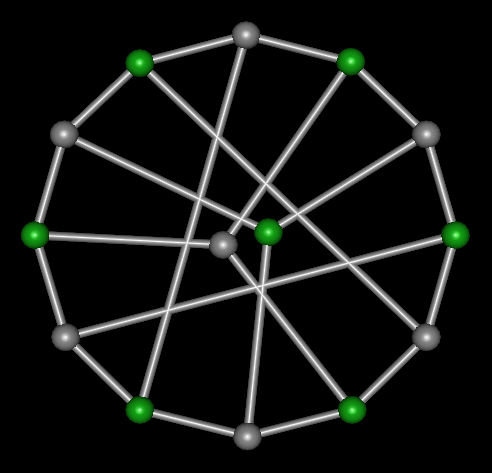
\includegraphics[width=0.4\textwidth]{img/bondymurphyg3.png}
\label{fig:example-bondymurphyg3}
\caption{Grafo de Bondy-Murphy $G_3$, $n=14$, $k=7$}
\end{figure}


\section{O grafo de Bondy-Murphy $G_4$}
Para o grafo de Bondy-Murphy $G_4$~\cite{cite:example-bondy} com $n=16$
vértices.

\begin{figure}[htb]
\centering
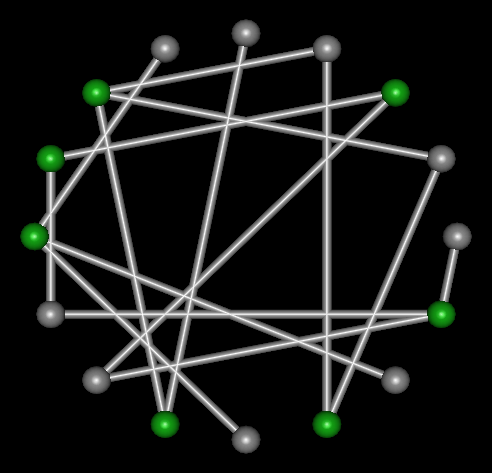
\includegraphics[width=0.4\textwidth]{img/bondymurphyg4.png}
\label{fig:example-bondymurphyg4}
\caption{Grafo de Bondy-Murphy $G_4$, $n=16$, $k=7$}
\end{figure}


\section{O grafo de Ramsey $R(4,4)$}
Para o grafo de Ramsey $R(4,4)$~\cite{cite:example-ramsey} com $n=17$
vértices.

\begin{figure}[htb]
\centering
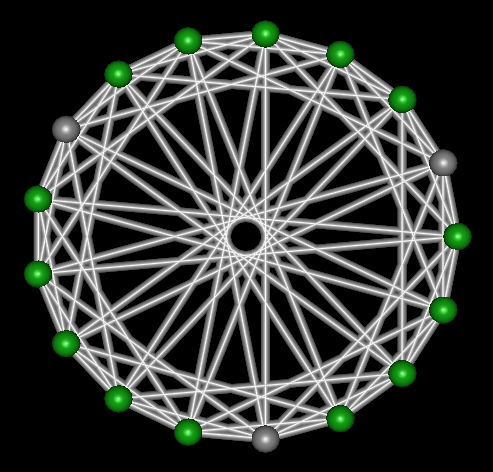
\includegraphics[width=0.4\textwidth]{img/ramsey.png}
\label{fig:example-ramsey}
\caption{Grafo de Ramsey $R(4,4)$, $n=17$, $k=14$}
\end{figure}


\section{O grafo de Folkman}
Para o grafo de Folkman~\cite{cite:example-folkman} com $n=20$
vértices.

\begin{figure}[htb]
\centering
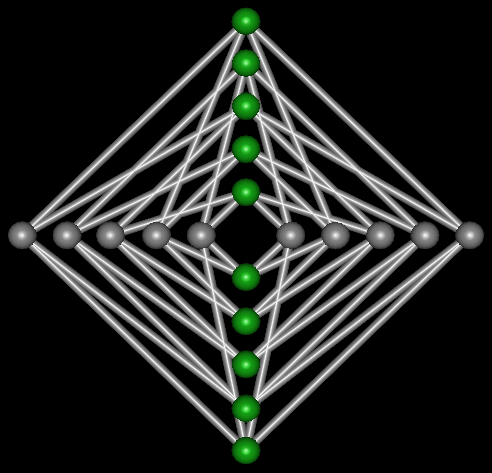
\includegraphics[width=0.4\textwidth]{img/folkman.png}
\label{fig:example-folkman}
\caption{Grafo de Folkman, $n=20$, $k=10$}
\end{figure}


\section{O dodecaedro}
Para o dodecaedro~\cite{cite:example-plato} com $n=20$ vértices.

\begin{figure}[htb]
\centering
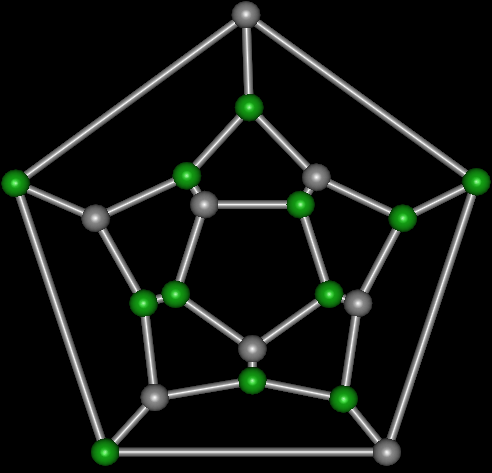
\includegraphics[width=0.4\textwidth]{img/dodecaedro.png}
\label{fig:example-dodecaedro}
\caption{Dodecaedro, $n=20$, $k=12$}
\end{figure}

\section{O grafo de Tutte-Coxeter}
Para o grafo de Tutte-Coxeter~\cite{cite:example-tutte} com $n=30$
vértices.

\begin{figure}[htb]
\centering
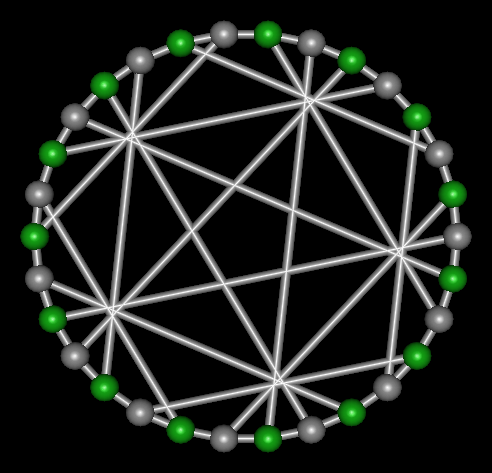
\includegraphics[width=0.4\textwidth]{img/tutte.png}
\label{fig:example-tutte}
\caption{Grafo de Tutte-Coxeter, $n=30$, $k=15$}
\end{figure}


\section{O grafo de Thomassen}
Para o grafo de Thomassen~\cite{cite:example-thomassen} com $n=34$
vértices.

\begin{figure}[htb]
\centering
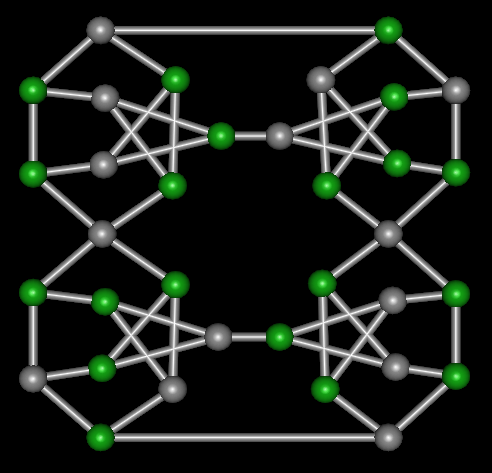
\includegraphics[width=0.4\textwidth]{img/thomassen.png}
\label{fig:example-thomassen}
\caption{Grafo de Thomassen, $n=34$, $k=20$}
\end{figure}


\section{O grafo de Berge}
Para o grafo de Berge~\cite{cite:example-berge} com $n=60$ vértices.

\begin{figure}[htb]
\centering
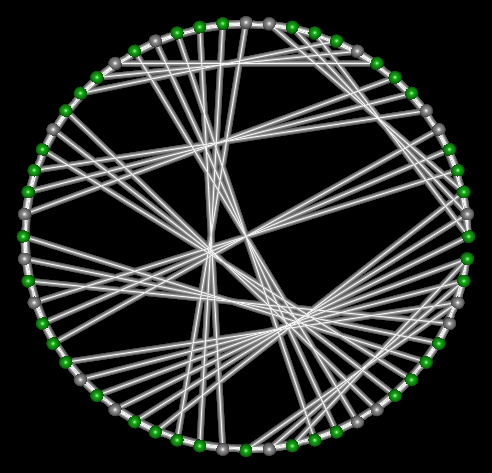
\includegraphics[width=0.4\textwidth]{img/berge.png}
\label{fig:example-berge}
\caption{Grafo de Berge, $n=60$, $k=40$}
\end{figure}


\section{O grafo de Witzel}
Para o grafo de Witzel~\cite{cite:example-witzel} com $n=450$
vértices.

\begin{figure}[htb]
\centering
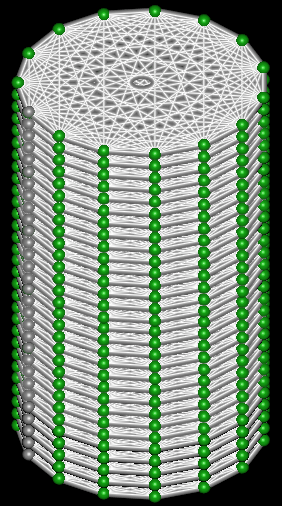
\includegraphics[width=0.4\textwidth]{img/witzel.png}
\label{fig:example-witzel}
\caption{Grafo de Witzel, $n=450$, $k=420$}
\end{figure}

